% !TeX root = ../sustechthesis-example.tex

\chapter[基于Isaac平台的深度学习训练实践]{基于Isaac平台的深度学习训练实践}
关于强化学习控制的整体理念流程在第\ref{section:rl_based_control}节中已经进行了介绍。对于具体的实现平台和代码实现案例在第\ref{section:isaac_gym}节和第\ref{section:legged_gym}节中也进行了说明。本节将给出一些实际进行RL训练的案例,以建立对实际RL训练的整体流程性认识。

\section[用legged\_gym例程库训练ANYmal-c]{用legged\_gym例程库训练ANYmal-c}
前几节所述的控制方法基本都是以ETH的足式机器人展开的,其中很多都是以ETH的ANYmal-c型号机器人为基础平台实现的。因此这里选择使用该型号的机器人进行实际的训练演示。
\subsection[训练脚本设置]{训练脚本设置}
首先需要按照官网的说明配置好相应的python、Isaac、CUDA、PyTorch等基本环境。然后将\emph{legged\_gym}的源码下载到本地安装。完成基本的配置后启动训练的操作是比较简单的。如下面代码\ref{code:sh_rl_train_script}所示,以我配置的环境为例。启动并进入到训练所需的conda环境(aconda,conda\_leg38是自定义的命令行别名),然后运行\emph{train.py}脚本并选择相应的训练目标即可。
\noindent
\begin{minipage}{\linewidth}
\begin{lstlisting}[language=python,caption={自定义的RL训练.sh快捷启动脚本},xleftmargin=20pt,label={code:sh_rl_train_script}]
aconda # 激活conda环境
conda_leg38 # 激活深度学习Python子环境 
# 转移到训练脚本目录
cd ~/legged_gym_env/legged_gym/legged_gym/scripts 
# 启动训练脚本,其中--task=xxx用来选择要开启的训练任务
python train.py --task=anymal_cpdj 
\end{lstlisting}
\end{minipage}

% \noindent
% \begin{minipage}[\linewidth]
%     \begin{lstlisting}[language=java, caption={自定义的RL训练.sh快捷启动脚本}, xleftmargin=20pt,label={code:sh_rl_train_script}]
        % aconda # 激活conda环境
        % conda_leg38 # 激活深度学习Python子环境
        % cd ~/legged_gym_env/legged_gym/legged_gym/scripts # 转移到训练脚本目录
        % python play.py --task=anymal_cpdj # 启动柜训练脚本,其中--task=xxx用来选择要开启的训练任务
%     \end{lstlisting}
% \end{minipage}
\subsection[训练过程信息]{训练过程信息}
启动训练后会打开一个监视器来观察仿真空间,同时再终端会输出学习过程的一阶基本信息。图片\ref{fig:legged_gym_train_demo_014}到\ref{fig:legged_gym_train_demo_495}展示了真个训练过程的几个节点。整个训练方式采用基于游戏的模式进行\cite[p3]{Rudin_Hoeller_Reist_Hutter_2021},初始时候所有的实例被初始化到不同的地形环境中并行地进行训练,随着训练的进行,表现好的会升级并被安排难度更高的任务,最终训练的结果是整个地图中所有的实例成一定的分布(各个位置都有一定的分布以保证最终的策略可以较好地处理所有的地形情况和任务难度)。

\begin{figure}
    \centering
    % \subcaptionbox{\emph{legged\_gym} 终端输出信息。\label{fig:legged_gym_train_demo_info}}
    % {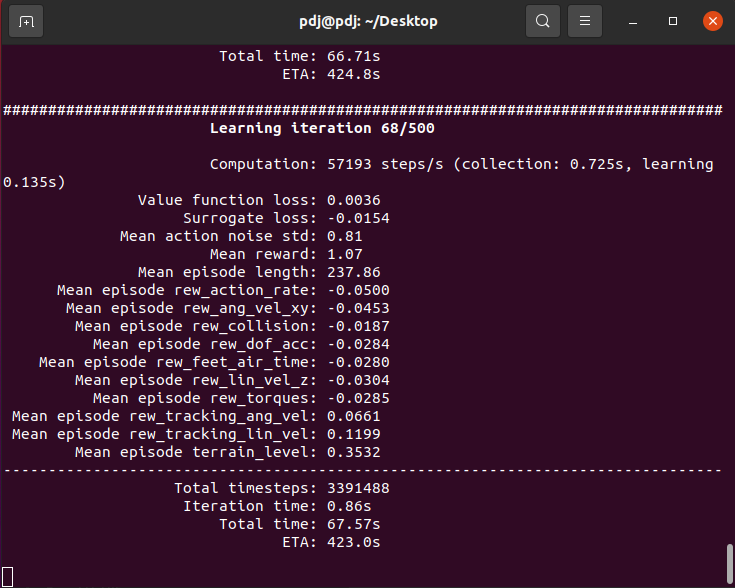
\includegraphics[width=0.47\linewidth]{legged_gym_train_demo_info.png}}
    \subcaptionbox{\emph{legged\_gym} 第14/500次迭代。\label{fig:legged_gym_train_demo_014}}
    {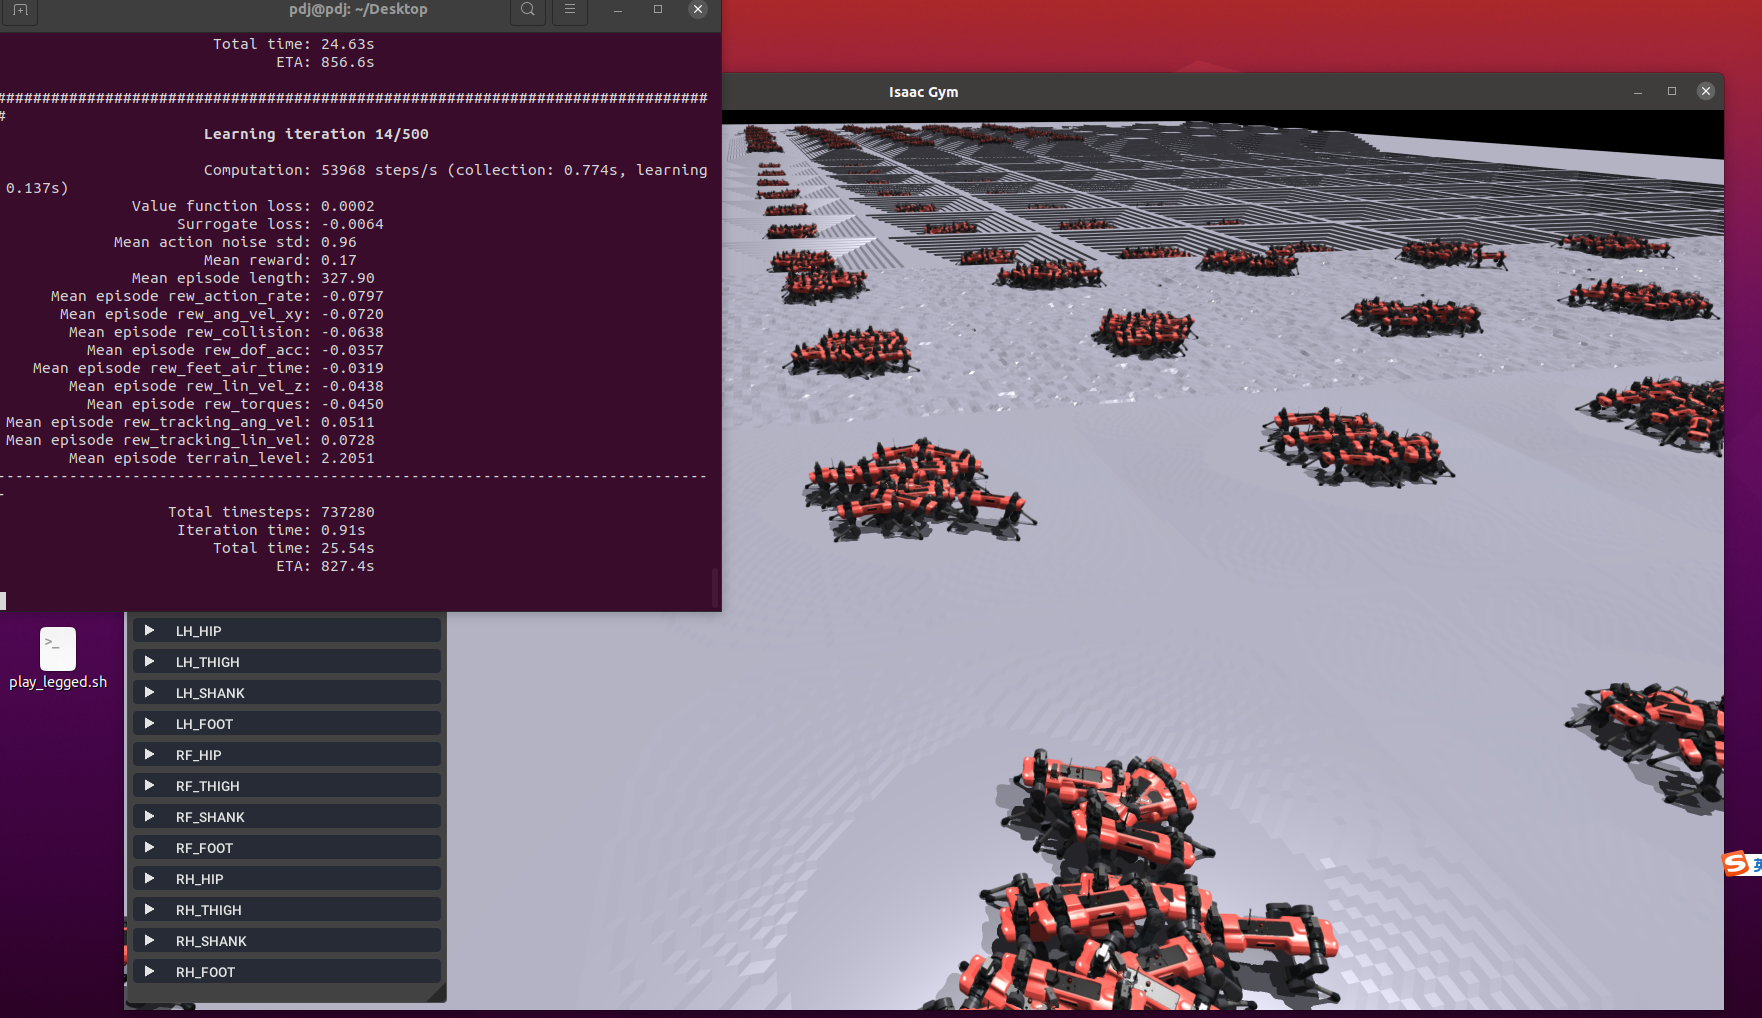
\includegraphics[width=0.47\linewidth]{legged_gym_train_demo_014.png}}
    \subcaptionbox{\emph{legged\_gym} 第200/500次迭代。\label{fig:legged_gym_train_demo_200}}
    {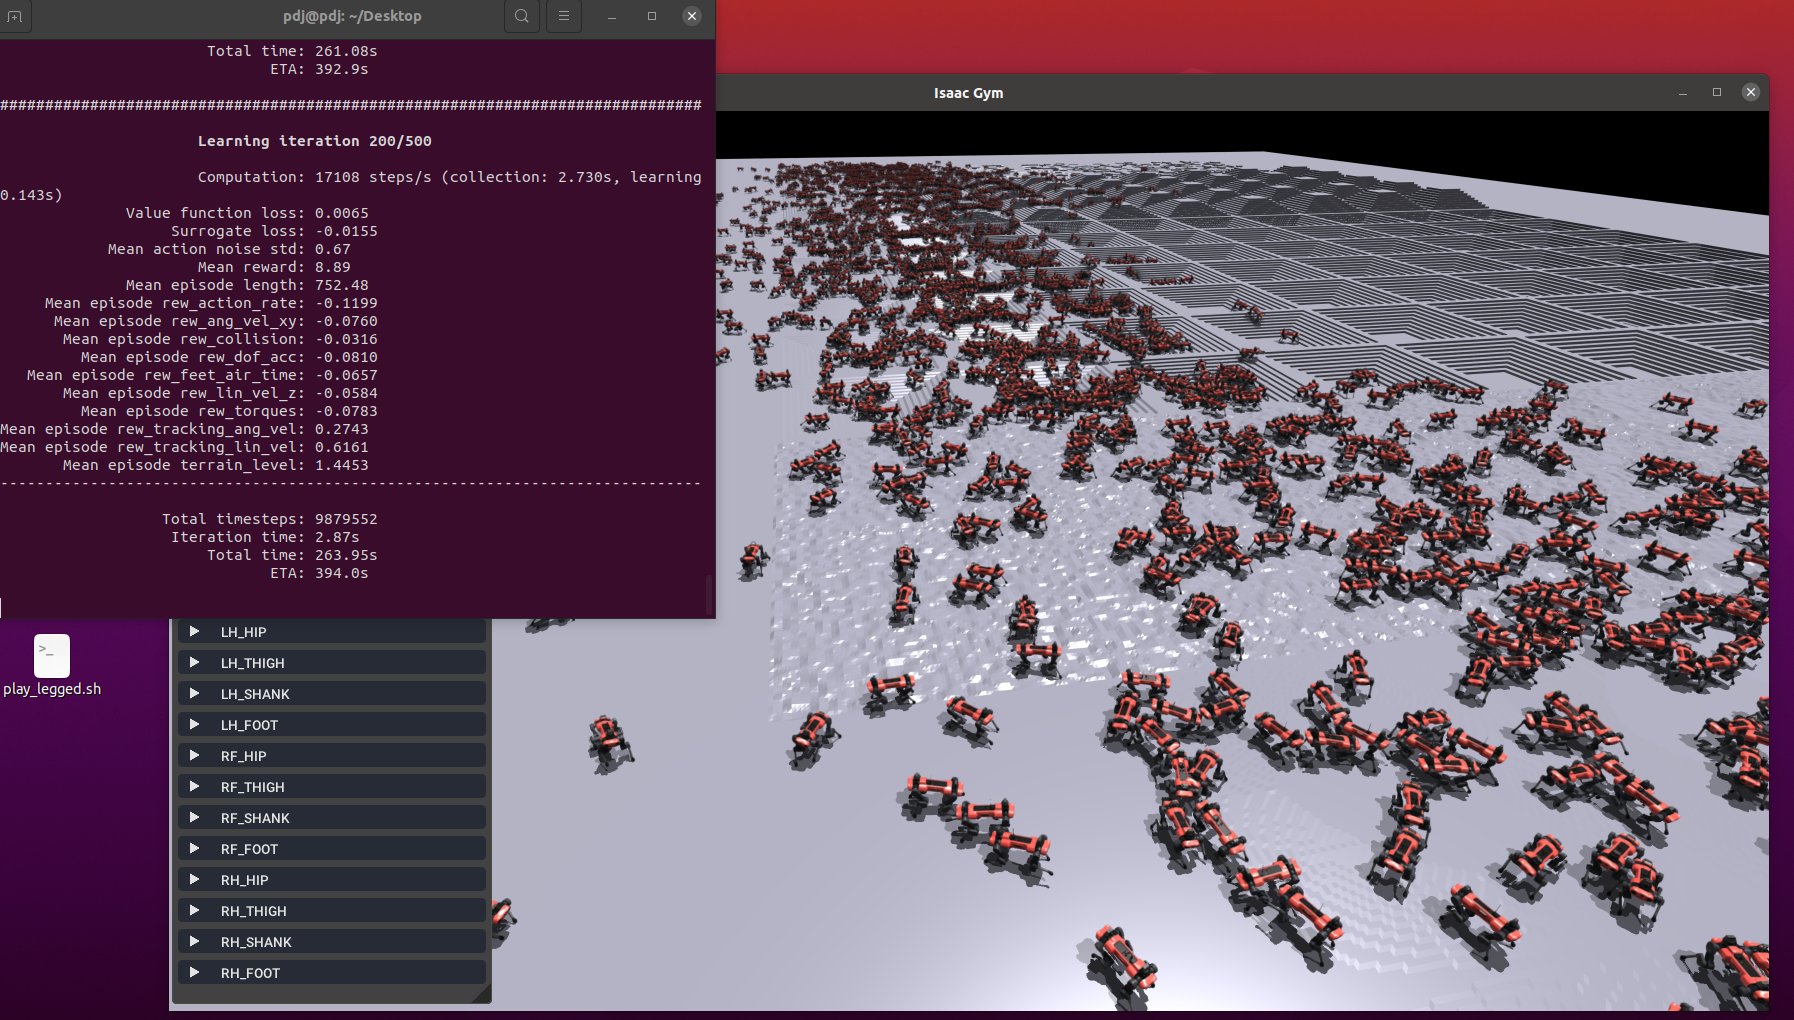
\includegraphics[width=0.47\linewidth]{legged_gym_train_demo_200.png}}
    \subcaptionbox{\emph{legged\_gym} 第350/500次迭代。\label{fig:legged_gym_train_demo_350}}
    {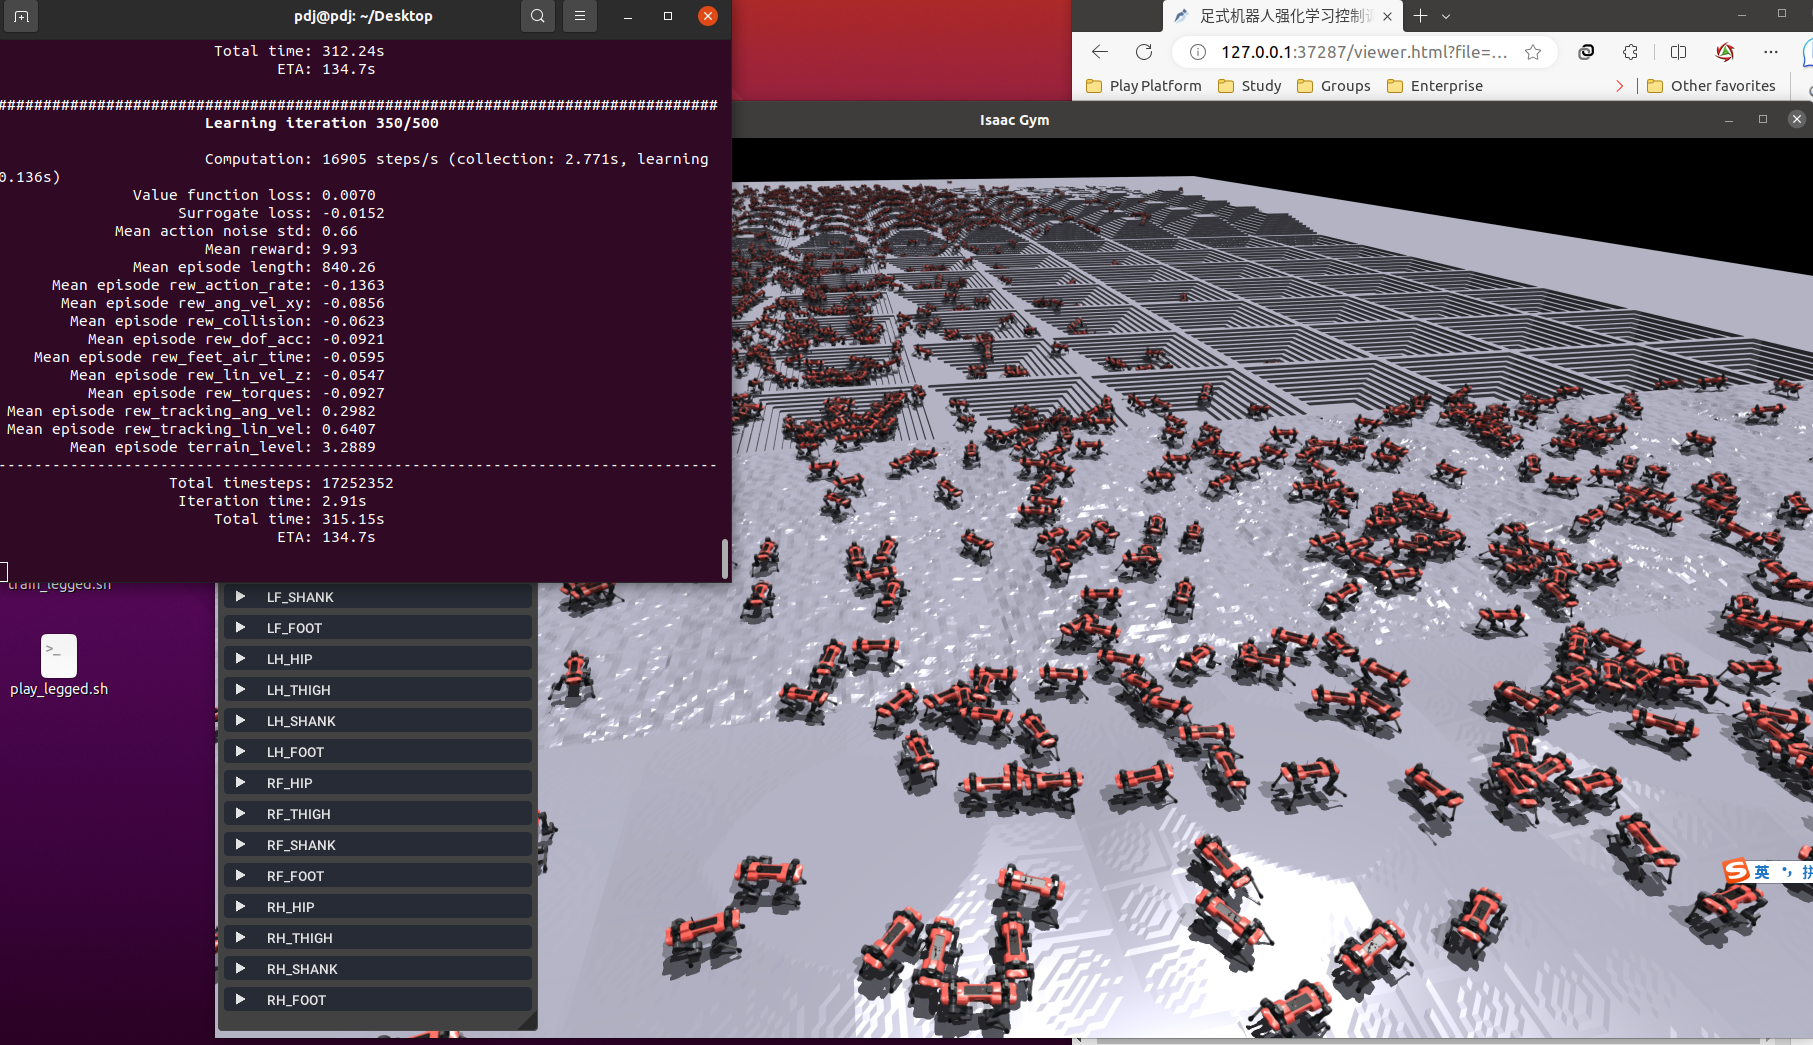
\includegraphics[width=0.47\linewidth]{legged_gym_train_demo_350.png}}
    \subcaptionbox{\emph{legged\_gym} 第495/500次迭代。\label{fig:legged_gym_train_demo_495}}
    {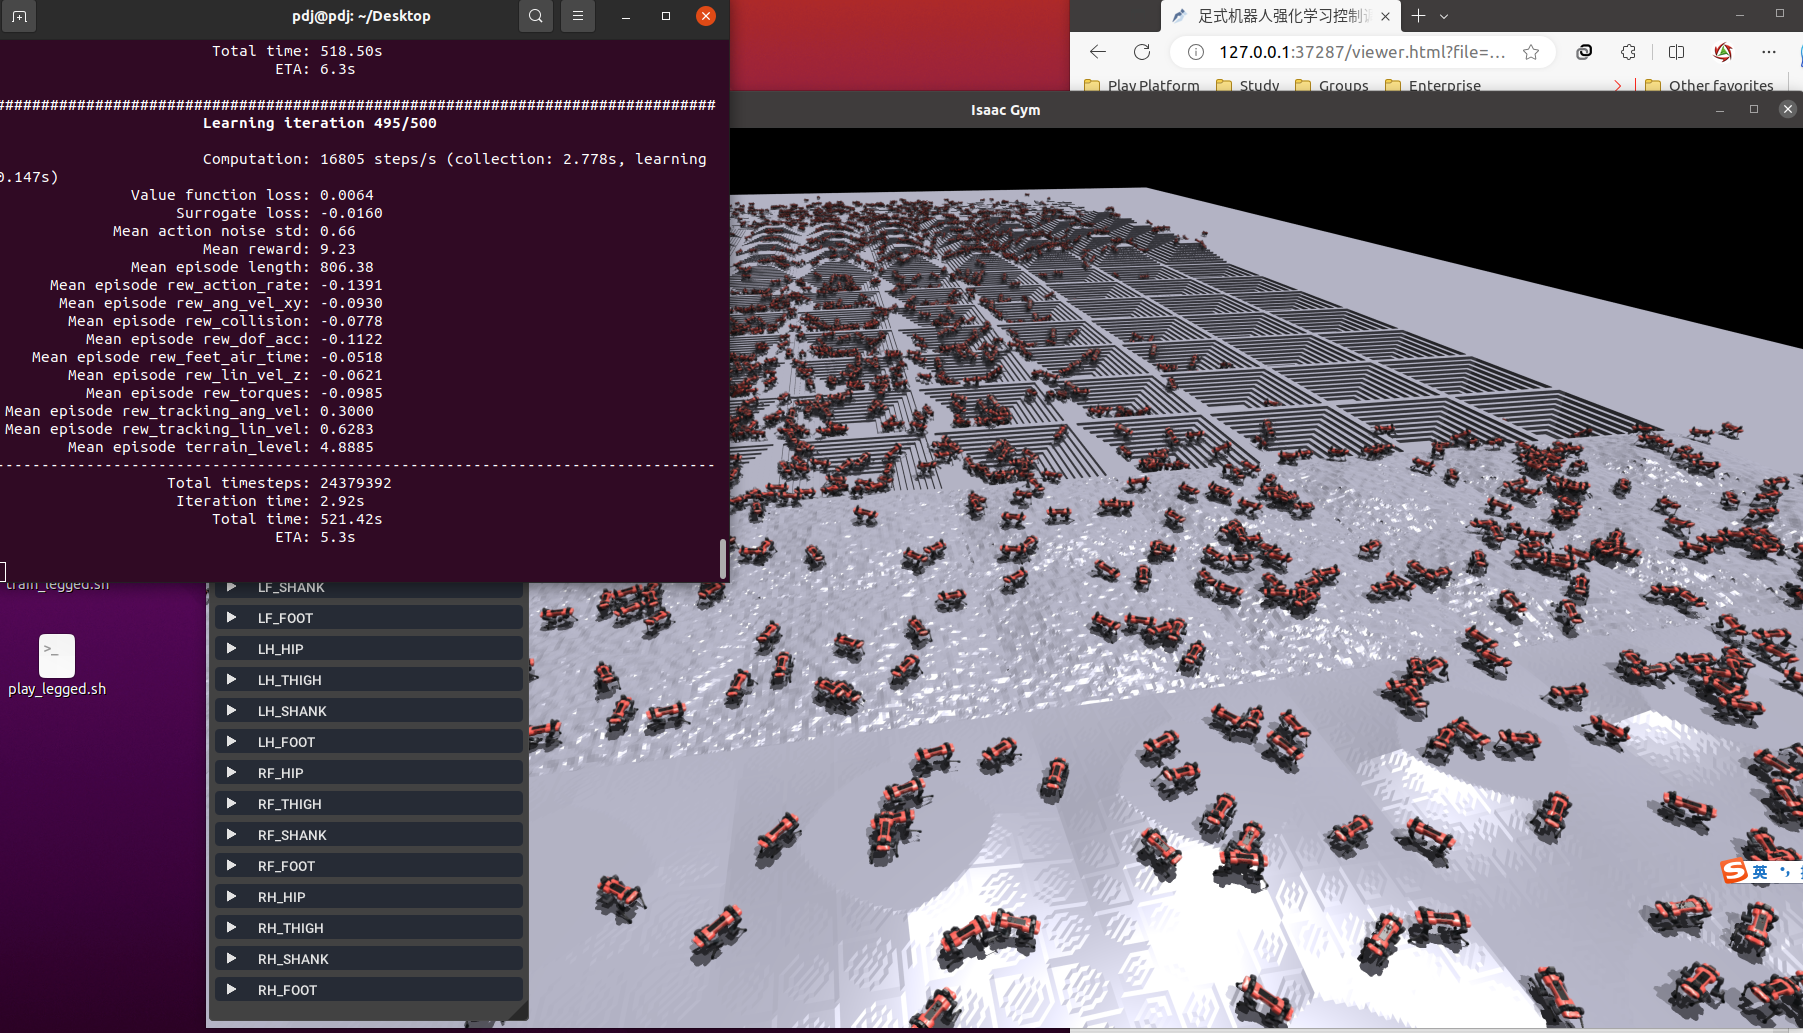
\includegraphics[width=0.47\linewidth]{legged_gym_train_demo_495.png}}
\end{figure}

\subsection[训练结果输出和重演测试]{训练结果输出和重演测试}
完成训练后启动训练的结果重演测试也是比较简单的。如下面代码\ref{code:sh_rl_play_script}所示,以我配置的环境为例。启动并进入到训练所需的conda环境(aconda,conda\_leg38是自定义的命令行别名),然后运行\emph{play.py}脚本并选择相应的训练目标即可。
\noindent
\begin{minipage}{\linewidth}
\begin{lstlisting}[language=python,caption={自定义的RL重演.sh快捷启动脚本},xleftmargin=20pt,label={code:sh_rl_play_script}]
aconda # 激活conda环境
conda_leg38 # 激活深度学习Python子环境
# 转移到训练脚本目录
cd ~/legged_gym_env/legged_gym/legged_gym/scripts 
# 启动训练脚本,其中--task=xxx用来选择要开启的训练任务
python play.py --task=anymal_cpdj 
\end{lstlisting}
\end{minipage}

\begin{figure}
    \centering
    \caption{\emph{legged\_gym} 采用训练好的策略控制机器人在仿真环境重演测试:整体上训练得到的策略已经能完成对不同地形的适应。}
    \label{fig:legged_gym_play_demo_view0}
    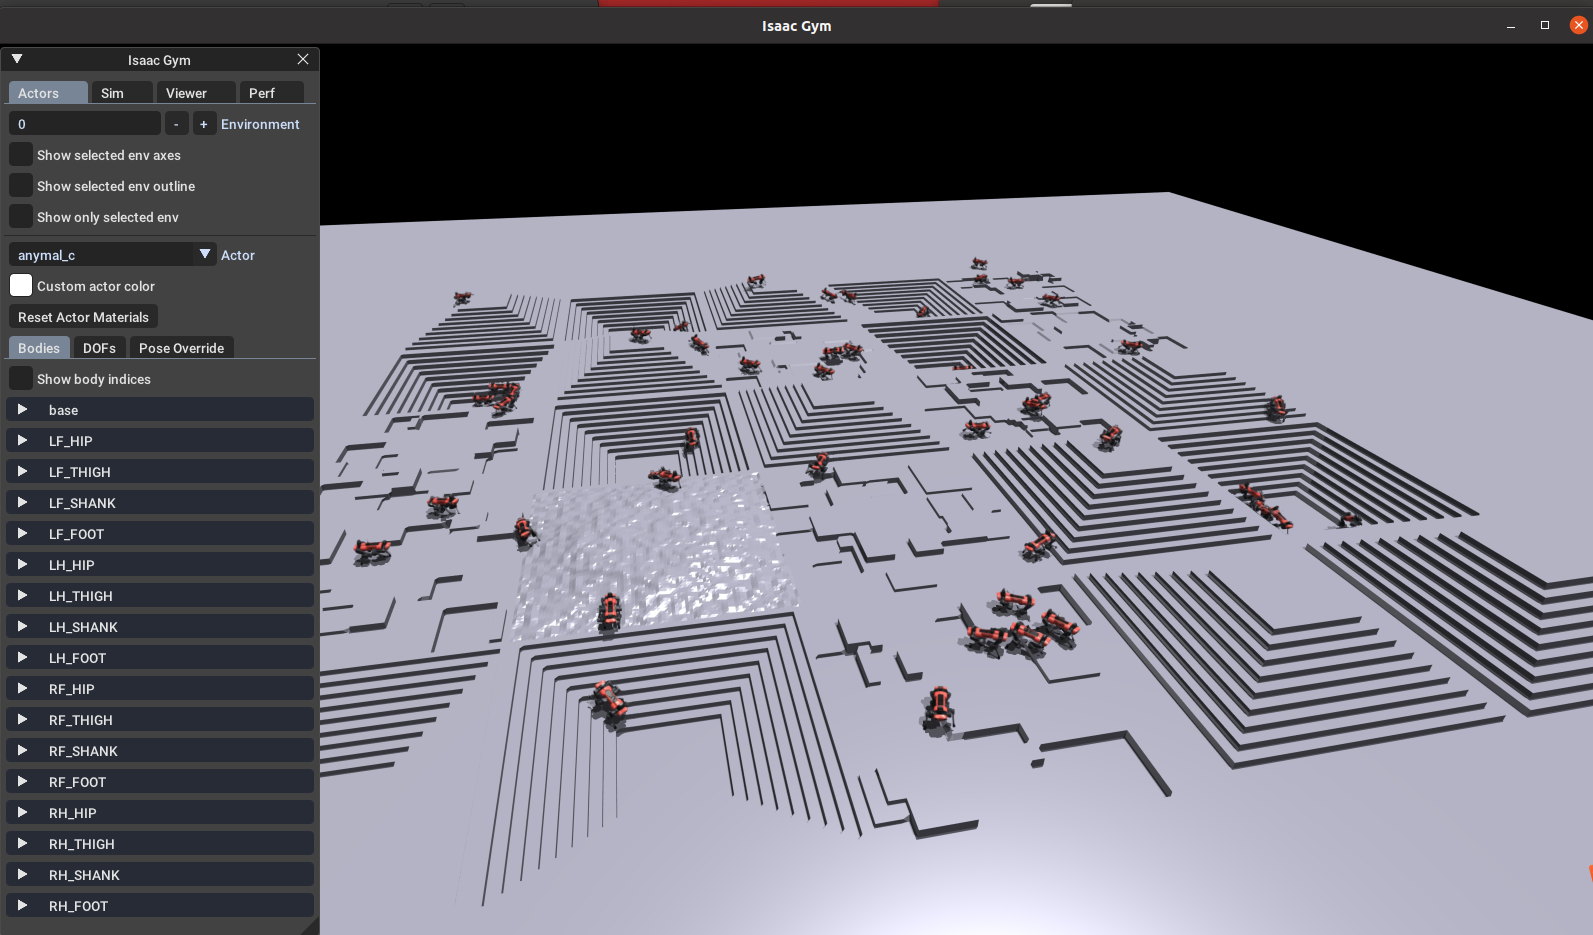
\includegraphics[width=1.0\linewidth]{legged_gym_play_demo_view0.png}
\end{figure}


如图\ref{fig:legged_gym_play_demo_view0}所示,用训练好的策略控制机器人在仿真环境中重演测试。可以看到机器人基本上已经能够无失误地应对各种地形环境,完成诸如上下楼梯、光滑地面行走、崎岖地面行走等任务了。

\begin{figure}
    \centering
    \caption{\emph{legged\_gym} 采用训练好的策略控制机器人在仿真环境重演测试:在完成某些地形情况下的任务时可能会出现犹豫、停顿甚至失败跌倒。}
    \label{fig:legged_gym_play_demo_view1}
    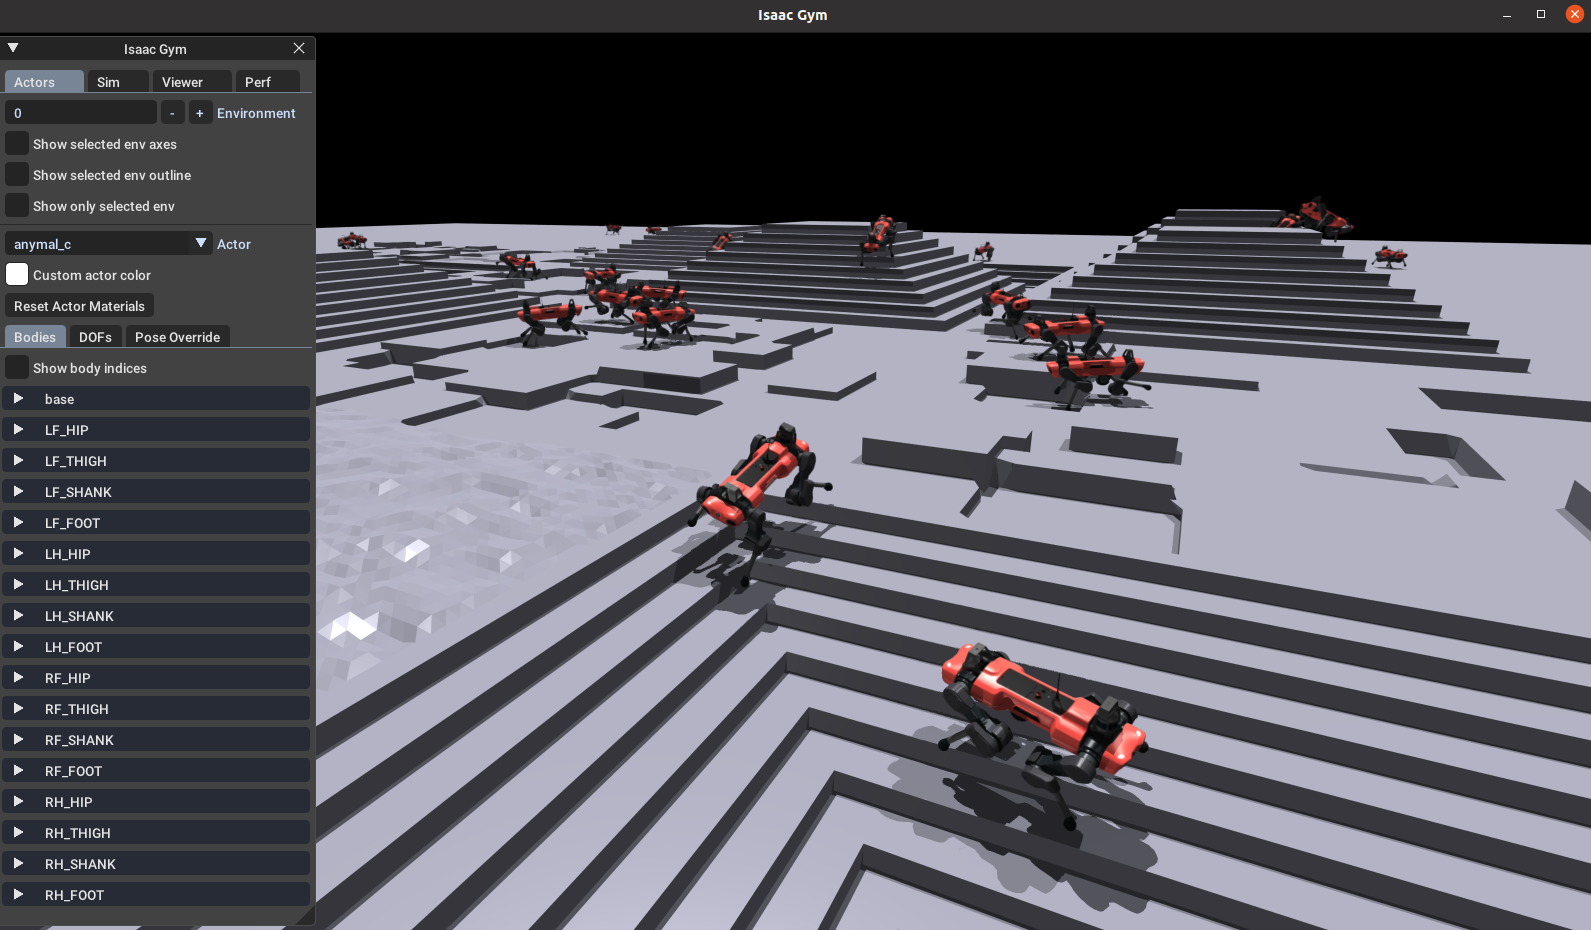
\includegraphics[width=1.0\linewidth]{legged_gym_play_demo_view1.png}
\end{figure}

不过,在面对较难任务时他们可能会犹豫、停顿甚至失败跌倒,如图\ref{fig:legged_gym_play_demo_view1}所示。这些问题可以通过设计更优的奖励机制进行训练、结合更多传感信息进行训练和部署、与传统控制结合起来控制等方式来进行解决。比如前面第\ref{section:rl_robust_in_wild}节介绍的,在这篇文献\cite[p4]{Miki_Lee_Hwangbo_Wellhausen_Koltun_Hutter_2022}中介绍了使用本体感知和外部感知融合,并使用经典的肢体动作生成器进行训练的方法,取得了很好的效果。

在完成重演测试的同时还会将PyTorch的策略结果转化成可用于C++实现的形式,输出路径为:\emph{../legged\_gym/logs/anymal\_cpdj/exported/policies/policy1.pt},输出格式为:\emph{.pt}文件。这为后续的\emph{仿真到实际(sim-to-real)}做了准备。

